\chapter{Preliminaries}\label{ch:preliminaries}

\section{Types of machine learning}
\label{sec:types-of-machine-learning}

There are different approaches to machine learning. In this section we will introduce a few of these approaches to give context for our research.

\todo{Possibly add semi-supervised learning as well?}

\subsection{Supervised learning}

Supervised learnin\cite{mohri_foundations_2012} is a type of machine learning that always uses a labeled dataset. This means that for each point in the dataset we already know what class or rank it belongs to. It is the common type of learning used with problems that require classification, regression or ranking. The known samples are used to train a model and to make predictions for data points that the model has not seen yet.

An example would be making predictions about images of animals. Each image would be labeled with the type of animal that is in the picture. We would be learning our models using that data to be able to predict the type of animals in pictures that the model has never seen before.

\subsection{Unsupervised learning}

This subset of machine learning focuses on training models with unlabeled data. Examples of problems that use this type of learning are clustering and dimensionality reduction. For unsupervised methods it is hard to measure the performance quantitatively because there are no labels to compare the results to.

An example of this type would be clustering people by known information like age, education or income. The goal here is to split the dataset based on information that is similar between the points. So only the points from the dataset are used to come to a result, there is no previous knowledge about the data that can be used.

\subsection{Self-supervised learning}

The type of machine learning that we use in this thesis is a form of self-supervised learning\cite{doersch_multi-task_2017}. This means that we generate our own labels from a dataset without any manual work required. This is possible by removing or modifying part of the input data and then learn a model to recover the original data. We can measure the performance based on the difference between the original data and the result. This type of learning can be seen as a combination of unsupervised and supervised learning.

An example is a model that tries to predict words in a certain context. We have a sentence: 'The most popular food from France is the croissant'. We can then leave out the word 'croissant' and train a model to predict the word based on the words surrounding it.

\todo{Add section about recurrent neural networks for completeness?}

\section{Transformers}
\label{sec:transformers}

The type of model used in our research is a transformer. In this section we will introduce the attention mechanism, explain how this is used in different types of transformers and what kind of transformer we are using.

\subsection{Vanilla transformers}

In 2017 Vaswani et al.\cite{vaswani_attention_2017} introduced the transformer model. A type of sequence to sequence model that uses an attention mechanism as the main building block. This allowed them to increase parallelisation and reach a new state of the art in the context of language translations.

\subsubsection{Architecture}

The transformer model uses the same encoder-decoder structure used in the models it was compared to in the original paper\cite{bahdanau_neural_2016, cho_learning_2014}. This means that the model consists of two parts: an encoder and a decoder.

The encoder takes an input representation $(x_1,...x_n)$ and transforms this to an intermediary representation $(z_1,...z_n)$. This intermediary representation is then used as input for the decoder to create an output $(y_1,...,y_n)$.

\begin{figure}[h]
\caption{The original transformer architecture from \cite{vaswani_attention_2017}}
\centering
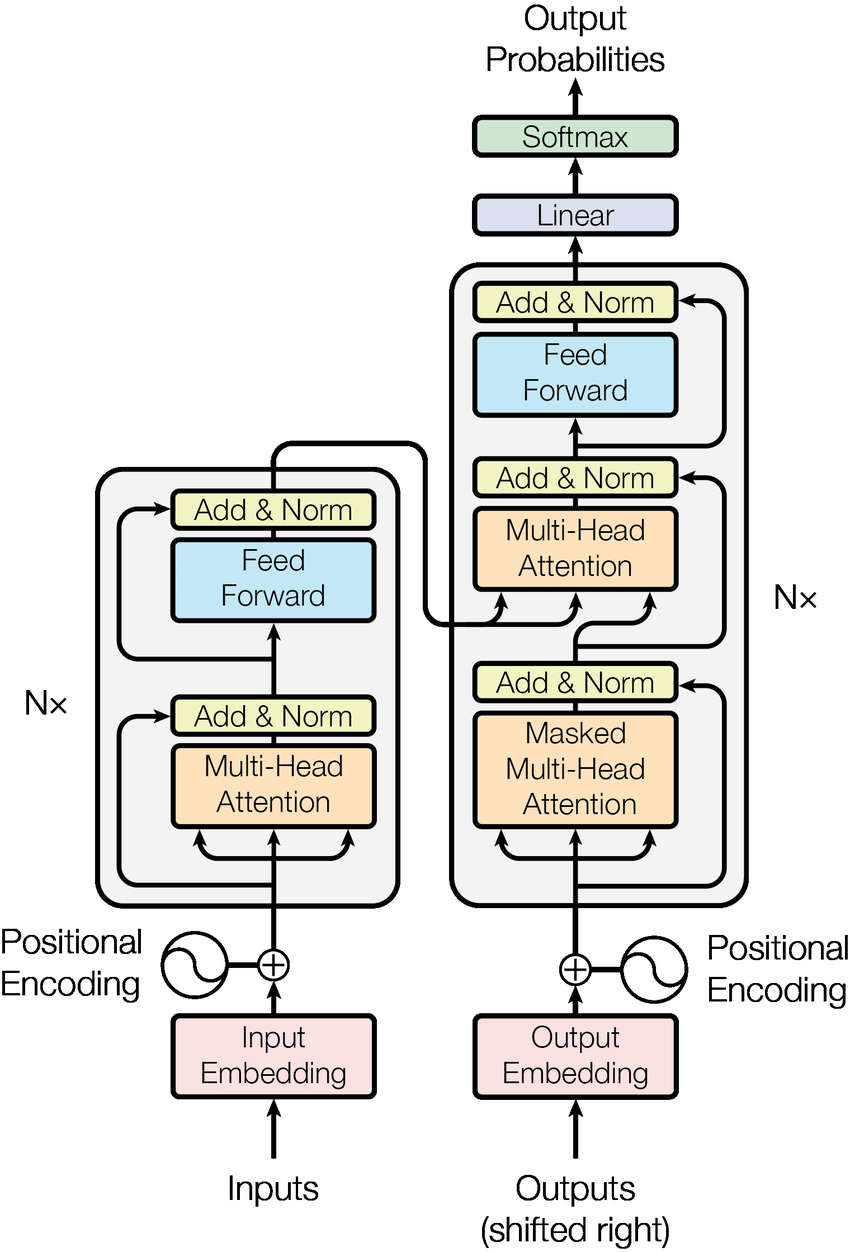
\includegraphics[width=0.5\textwidth]{../imgs/transformer.png}
\label{fig:transformer-architecture}
\end{figure}

\paragraph{Encoder}
The encoder part in the architecture is a stack of $N$ layers. All the layers are the same and consist of two sub-layers: the multi-head self-attention and a fully-connected feed-forward network (FFN) that is fully connected. After both sub-layers we apply layer normalisation\cite{ba_layer_2016} and add residual connections\cite{he_deep_2015} around the sub-layers. This means that the output of a layer in the encoder is calculated as follows: 
\begin{align*}
&selfAtt = LayerNorm(input + SelfAtt(input_q, input_k, input_))\\
&out = LayerNorm(selfAtt + FFN(selfAtt))
\end{align*}


\paragraph{Decoder}
Similar to the encoder the decoder is a stack of $N$ layers. Compared to the encoder it adds a third sub-layer that applies multi-head cross attention to the output from the encoder layers and the first sub-layer of the decoder. In comparison to the encoder the first self-attention sub-layer we mask out earlier positions in the output sequence to stop predictions for a certain position $i$ to depend on the outputs at the positions before position $i$. The residual connections and layer normalisation on each sub-layer is identical to the architecture of the encoder. This results in the following calculations for each decoder layer: 
\begin{align*}
&selfAtt = LayerNorm(input + MaskedSelfAtt(in_q, in_k, in_v))\\
&crossAtt = LayerNorm(selfAtt + CrossAtt(selfAtt_q, enc_k, enc_v))\\
&out = LayerNorm(crossAtt + FFN(crossAtt))
\end{align*}

The final layers consist of a linear fully connected neural network and a Softmax layer. This allows us to have a higher number of possible outputs than the size of the input and output embeddings since it projects the output of the decoder part into a probability vector.

\paragraph{Attention}

As explained in the previous paragraphs we use attention in the model. This mechanism, which takes query, keys and values vector as input, outputs a vector containing a weighted sum of the values. Each of the output values uses a weight that is calculated using a compatibility  function of the query and the key in each position.

The attention mechanism from \cite{vaswani_attention_2017} is called 'Scaled Dot-Product Attention' and calculates attention using matrices $Q$ (queries), $K$ (keys) of dimensiion $d_k$ and $V$ (values) of dimension $d_v$ that consist of multiple vectors:
\begin{align*}
&Attention(Q, K, V) = softmax(\frac{QK^T} {sqrt(d_k)})V
\end{align*}

To be able to apply the attention to more than one representation space we use multi-headed attention. This uses $h$ parallel layers that all attend to a smaller part of the full dimension. In the case of the original papers $h = 8$ and the dimension of each attention head becomes $d_k = d_v = d_model / h = 64$. This makes the multi-headed attention similar to single-head attention with the full dimension when we look at the computational cost.

To do this we learn different linear projections that we project all queries, keys and values to.  All the separate outputs of the different attention heads are concatenated and projected which gives us the final output.

\begin{align*}
&MultiHead(Q, K, V) = Concat(head_1, ..., head_h)W^O
& where head_i = Attention(QW_i^Q, KW_i^K, VW_i^V
\end{align*}


\subsection{Vision transformers}

\cite{dosovitskiy_image_2021}

Transformers can be used for images too

to input the images we reshape the images into flattened 2 patches
so we go from 

$x < R^HxWxC to x_p < R^N x (P^2.C)$ where $(H, W)$ is the resolution of the image, $C$ is the number of channels and $(P,P)$ is the patch resolution
and $N = HW/P^2$ the number of patches


\subsection{Linear transformers}

\cite{katharopoulos_transformers_2020}

transformers are RNNs

this changes the softmax to a linear calculation so that the complexity of the the transformers is decreased

\iffalse

\fi


\section{Image inpainting}
\label{sec:image-inpainting}



\iffalse

\fi


\section{Anomaly detection}
\label{sec:anomaly-detection}



\iffalse

\fi



\iffalse
- Unsupervised learning
- Anomaly detection
- Transformers
\fi